\documentclass{IEEEcsmag}

\usepackage[colorlinks,urlcolor=blue,linkcolor=blue,citecolor=blue]{hyperref}

\usepackage{upmath}
\usepackage{amssymb}
\usepackage{amsmath}
\usepackage{array}
\newcolumntype{P}[1]{>{\centering\arraybackslash}p{#1}}

\jvol{XX}
\jnum{XX}
\paper{8}
\jmonth{May/June}
\jname{Computing in Science and Engineering}
\pubyear{2021}
\newtheorem{theorem}{Theorem}
\newtheorem{lemma}{Lemma}

\setcounter{secnumdepth}{0}

\begin{document}

\sptitle{Department: Head}
\editor{Editor: Name, xxxx@email}

\title{PyExaFMM: Designing a high-performance particle fast multipole solver in Python with Numba}

\author{S. Kailasa}
\affil{Department of Mathematics, University College London}

\author{T. Wang}
\affil{Department of Mechanical and Aerospace Engineering, The George Washington University}

\author{\text{L}. A. Barba}
\affil{Department of Mechanical and Aerospace Engineering, The George Washington University}

\author{T. Betcke}
\affil{Department of Mathematics, University College London}

\markboth{Department Head}{Paper title}

\begin{abstract}
The particle fast multipole method is a good case study for understanding the efficacy of Python for developing high-performance software for non-trivial algorithms, due its reliance on a hierarchical tree data structure. In this paper we describe the mathematical and software engineering techniques used to extract performance for PyExaFMM, a Python based solver for the particle fast multipole method, accelerated with Numba, designed to be run on single-node multicore architectures. We report that we achieve runtimes within $\mathcal{O}(10)$ of the state of the art C++ implementation, with comparable accuracy and memory footprint for three dimensional problems in double precision.
\end{abstract}

\maketitle
\chapterinitial{CPython is the original and most} popular implementation of the Python programming language, which is both dynamically typed and interpreted. CPython was designed with safety and developer productivity in mind, rather than high-performance computing [HPC]. Dynamic typing forces objects to be passed through the interpreter loop at runtime, and applications are restricted to a single thread via a `global interpreter lock' [GIL] to ensure thread safety. However, Python's popularity has lead to the development of numerous open-source tools for HPC with CPython, that allow users to bypass the interpreter, develop multithreaded applications, and even deploy source code written in Python to GPUs.

PyExaFMM\footnote{https://www.github.com/exafmm/pyexafmm} is a solver for the particle fast multipole method [FMM]. It was designed to test the efficacy of Numba, a `just-in-time' [JIT] compiler, for developing HPC applications in CPython. Building on the success of the ExaFMM project's comparable C++ implementation \cite{Wang2021}, we wanted to test whether we could retain the productivity benefits of working in Python while achieving performance comparable to compiled languages.  The FMM consists of a recursive loop through a hierarchical data structure. Representing computations and data efficiently while retaining performance is challenging, therefore it offers a good benchmark for studying the efficacy of Python and Numba for developing efficient software for complex algorithms.

Numba appears to offer an excellent development framework for overcoming the performance problems of Python. It bypasses the interpreter for operations involving loops over Numpy arrays and numeric scalars, translating Python source code into efficient platform-dependent machine code using the LLVM infrastructure. LLVM applies hardware dependent optimizations such as single-instruction multiple data [SIMD] vectorization over loops, to the intermediate bytecode representation [IR] produced by Numba. Bypassing the Python interpreter in this way makes Numba compiled functions competitive with compiled languages such as C++ and Fortran. Numba is a `drop-in' tool, functions or classes are marked for JIT compilation with a decorator, and `polymorphic dispatching' picks up input and output type data from the objects arguments at runtime - compiling the function for these types. Therefore Numba fits easily into existing Python projects. Numba has been extended with efficient implementations of many of the array manipulation and linear algebra operations offered by Numpy, as well as multithreading functionality via iterations over a parallel range iterator, reminiscent of OpenMP's parallel for loops. Furthermore, Numba supports the writing of Python kernels for AMD and NVidia GPUS, and is fully integrated with the CuPy library. Numba therefore provides a framework for developing cross-platform, heterogenous, applications using only Python source code. However, developing applications in Numba still requires interaction with the Python interpreter to allocate data before passing to optimized functions, as well as to interact with non-optimized parts of the codebase involved in data-organization or calls to incompatible libraries.



- This paper consists of:
	- Brief intro to FMM algorithm (<1000 words)
	- Math methods, software design and parallelization strategies for achieving performance with Numba. (~2500 words)
	- Benchmarks wrt comparable C++ module (~1500 words)

\section{FAST MULTIPOLE METHODS}

% Larger figure
\begin{figure*}
	\centerline{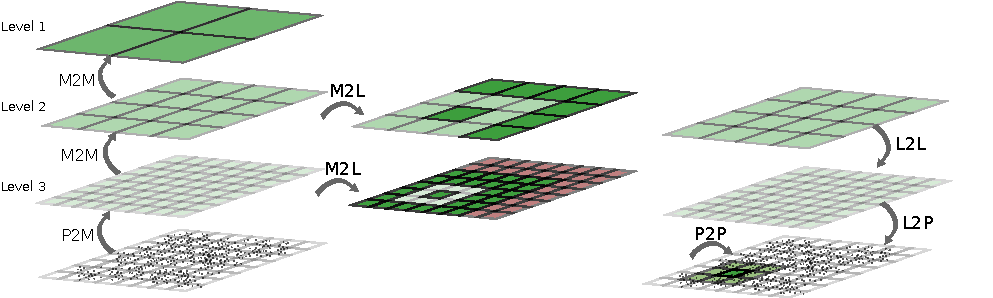
\includegraphics {figures/algorithm.pdf}}
	\caption{algorithm}
	\label{fig:agorithm}
\end{figure*}

\begin{figure*}
	\centerline{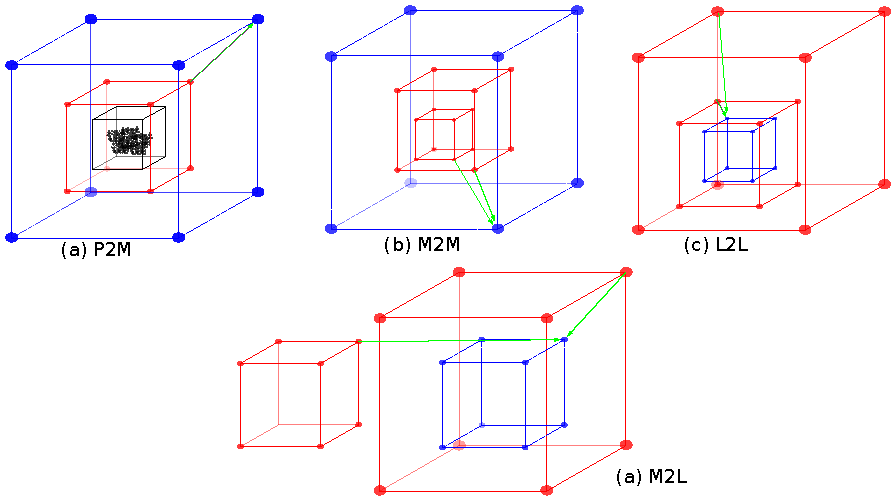
\includegraphics {figures/operators.pdf}}
	\caption{The operators of the KIFMM. Equivalent surfaces are shown in red, check surfaces in blue, and the charged points in black. Surfaces are plotted with 8 quadrature points, one at each vertex.}
	\label{fig:operators}
\end{figure*}
% Smaller figure
\begin{figure}
	\centerline{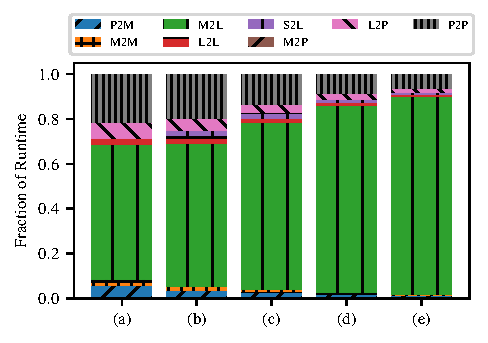
\includegraphics {figures/operator_runtimes.pdf}}
	\caption{Foo bar}
	\label{fig:operator_runtimes}
\end{figure}


\section{TECHNIQUES FOR ACHIEVING PERFORMANCE}

 Python's expressiveness allows PyExaFMM to be a concise library, consisting of $\sim$3,000 lines of code, in comparison to comparable single-node C++ implementations ExaFMM-T ($\sim$7000 lines) \cite{Wang2021} or TBFMM ($\sim$20,000) \cite{Bramas2020}.
% foo


% \subsection{Numba}

% - What it is, where it's useful.
% 	- Fast machine code for simple functions
% 	- Simplified multithreading
% 	- GPU and CPU code from the same source.

% \subsection{Efficient Operators}

% - Parallelization strategies.

\begin{table*}
	\centering
	\caption{Relative error, runtime and peak memory consumption in comparison to the SOTA. Experiments run with $N=1,000,000$ points tested in two geometries: (1) distributed randomly in a cubic unit box, (2) distributed randomly on the surface of a sphere with unit radius, leading to $M$ leaves in their respective geometries, with a maximum of $150$ points per leaf, multipole and local expansions of order $p$, and a compression rank $k$ for PyExaFMM. Charge densities are chosen in the interval $[0, 1)$. Runtimes exclude tree building time. Reported to 3 significant figures after a single run.}
	\begin{tabular}{|*{10}{c|}}
		\hline
		& & &   & \multicolumn{2}{c|}{Runtime} & \multicolumn{2}{c|}{Peak Memory} & \multicolumn{2}{c|}{Relative Error}\\
		\hline
		$k$ & $M$ &$p$ &  Geometry   &   PyExaFMM  &  ExaFMM-T &    PyExaFMM  &  ExaFMM-T  &   PyExaFMM  &  ExaFMM-T\\
		\hline
		10 & 17,017 & 6   &   Sphere  &  $10.6 \pm 0.1$ s & $0.41 \pm 0.04$ s  &  2.96 GB  &   2.34 GB  & 1.00e-4 & 8.75e-5\\
		 & 32,768 &    &   Random  &  $13.2 \pm 0.2$ s &  $0.41 \pm 0.05$ s &  4.93 GB  &   2.98 GB  & 8.75e-5 & 7.66e-5\\
		 &  & 10   &   Sphere  &  $57.0 \pm 0.1$ s &  $1.78 \pm 0.04$ s  &  3.09 GB  &   3.22 GB  & 2.00e-6 & 2.86e-6\\
		 &  &    &   Random  & $131 \pm 2$ s &   $2.11 \pm 0.06$ s  &  4.93 GB  &   3.88 GB  & 1.71e-6 & 3.84e-6\\
%%%%
		100 & 17,017 & 6   &   Sphere  &  $10.6 \pm 0.1$ s & $0.41 \pm 0.04$ s  &  2.96 GB  &   2.34 GB  & 1.00e-4 & 8.75e-5\\
		 & 32,768 &    &   Random  &  $13.2 \pm 0.2$ s &  $0.41 \pm 0.05$ s &  4.93 GB  &   2.98 GB  & 8.75e-5 & 7.66e-5\\
		 &  & 10   &   Sphere  &  $57.0 \pm 0.1$ s &  $1.78 \pm 0.04$ s  &  3.09 GB  &   3.22 GB  & 2.00e-6 & 2.86e-6\\
		 &  &    &   Random  & $131 \pm 2$ s &   $2.11 \pm 0.06$ s  &  4.93 GB  &   3.88 GB  & 1.71e-6 & 3.84e-6\\
%%%%
		Full Rank & 17,017 & 6   &   Sphere  &  $10.6 \pm 0.1$ s & $0.41 \pm 0.04$ s  &  2.96 GB  &   2.34 GB  & 1.00e-4 & 8.75e-5\\
		 & 32,768 &    &   Random  &  $13.2 \pm 0.2$ s &  $0.41 \pm 0.05$ s &  4.93 GB  &   2.98 GB  & 8.75e-5 & 7.66e-5\\
		 &  & 10   &   Sphere  &  $57.0 \pm 0.1$ s &  $1.78 \pm 0.04$ s  &  3.09 GB  &   3.22 GB  & 2.00e-6 & 2.86e-6\\
		 &  &    &   Random  & $131 \pm 2$ s &   $2.11 \pm 0.06$ s  &  4.93 GB  &   3.88 GB  & 1.71e-6 & 3.84e-6\\
		\hline
	\end{tabular}
	\label{tab:performance}
 \end{table*}

Larger figure
\begin{figure*}
	\centerline{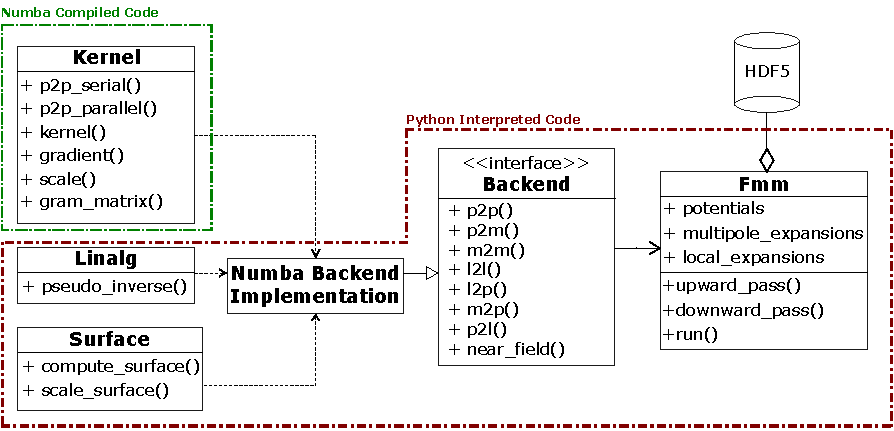
\includegraphics {figures/software.pdf}}
	\caption{Simplified UML model of all PyExaFMM components. Trees and operators are precomputed and stored in the HDF5 database. Except for the `Fmm' object which acts as the user interface, all other components are modules consisting of simple functions.}
	\label{fig:design}
\end{figure*}


% \section{PERFORMANCE}
% foo


% \section{CONCLUSION}

% foo

\section{ACKNOWLEDGMENT}

SK is supported by EPSRC Studentship 2417009.

\bibliography{pyexafmm}

\bibliographystyle{ieeetr}

\begin{IEEEbiography}{Srinath Kailasa}{\,}is a Graduate Student at UCL, currently pursuing a PhD in Computational Mathematics. He completed an MPhys in Physics (2017) and an MSc in Scientific Computing (2020) from Durham University and UCL respectively, interspersed with time as a Software Engineer in industry. His research interests are in high-performance and scientific computing. Contact him at srinath.kailasa.18@ucl.ac.uk.
\end{IEEEbiography}

\begin{IEEEbiography}{Tingyu Wang}{\,}is a PhD student in Mechanical Engineering at the George Washington University. Contact him at twang66@email.gwu.edu.
\end{IEEEbiography}

\begin{IEEEbiography}{Lorena. A. Barba}{\,}is a Professor of Mechanical and Aerospace Engineering at the George Washington University.  Contact her at labarba@email.gwu.edu.
\end{IEEEbiography}

\begin{IEEEbiography}{Timo Betcke}{\,}is Professor of Computational Mathematics at University College London. Is the lead investigator of the Bempp project, an open-source boundary element library. He studied Engineering in Germany as Undergraduate and then completed a PhD in Oxford in Numerical Analysis. From 2005 to 2006 he had various research positions until he became a Lecturer at UCL in 2011. Since 2018 he is a full Professor in the Department of Mathematics at UCL. Contact him at t.betcke@ucl.ac.uk.
\end{IEEEbiography}
\end{document}

